\documentclass{llncs}
\usepackage{graphicx}
\usepackage{amssymb}
\usepackage[numbers,sort]{natbib}
\usepackage{url}

\renewcommand\bibname{References}
\newcommand{\keywords}[1]{\par\addvspace\baselineskip
\noindent\keywordname\enspace\ignorespaces#1}
%
\begin{document}

\title{E-Lab: Web Based System for Automatic Assessment of
Programming Problems}

\author{Tomche Delev\inst{1} \and Dejan Gjorgjevikj\inst{1}}

\institute{Faculty of Computer Science and Engineering
\email{\{tomche.delev,dejan.gjorgjevikj\}@finki.ukim.mk}}


\maketitle


\begin{abstract}
\emph{E-Lab} is a system developed at Faculty of Computer Science and
Engineering for solving and auto-grading programming problems from introduction
to programming courses. The main goal is to simplify and improve the
organization and the process of solving programming problems from large group of
students in dedicated computer labs using centralized server. All the work from
the students is done in a web browser using a web-based code editor and
everything is stored, compiled and executed on the server. The system 
keeps records of all problem attempts from identified students which are used as
attendance records. All the problems and solutions are under version control
system (Git). The platform supports different types of problems in several
programming languages (C, C++, Java) and it's designed to be easily extended.

\keywords{Online submission, programming languages, automated assessment}
\end{abstract}

\section{Introduction}
Programming is one of the essential practical skills taught at introduction
level courses in computer science curricula. Mastering this skill can improve
students' chances in finding fair job and developing successful career. The
rewarding career and the constant raising of the market for programmers, makes
the computer science programs very popular among high school students. This,
results in larger number of students at the introductory classes with several
hundred students enrolled.

Programming is not an easy skill to develop. By some studies \cite{winslow1996programming}, mastering this
skill requires up to ten years. As easy as it seems, teaching basic programming
raises challenges to the academic stuff and good organization with the right
tools is required to tackle these challenges. Similarly to other practical
skills, good strategy for learning programming involves great amount of time
actually doing it. For introduction level courses involving some kind of
programming, this translates to solving a lot of basic algorithmic examples. To
incorporate this practice in the courses, the students organized in smaller
groups are required to spend considerable amount of time solving this kind of
programming problems organized in problem sets by the topic and held in
dedicated computer labs.

Several hundred students working on a set of problems every week, produces
thousands attempted solutions in form of source code that should be examined and
graded. In the current environment students work on PC workstations using simple
text editor or some kind of IDE for the programming language they use. They
save, compile and execute the solutions on their local machines. After they
finish, no records of their work is stored on server repository, so there is no
possibility for the instructors to examine and grade their solutions afterwards.
The time limit for each group of students is in the range of 90 to 120 minutes,
and the instructors usually have only up to 30 minutes to examine, test and
grade all the students of the group assigned to them (the group they are
tutoring) which is usually around 20, each with solutions for several problems.
These settings makes almost impossible for the instructors to quality assess the
students work, or if possible makes it a very dubious task.

The nature of the programming problems in great part of the introduction
programming courses is algorithmic. This makes it possible to develop a fairly
simple platform for creating problems, test cases and system for automatic
assessment and grading the solutions. Most algorithmic problems can be designed
to take some input from the standard input in some prescribed format, apply some
simple algorithm, and finally produce an output in some prescribed format and
print it on the standard output. Having this kind of problems we can take the
executable of the program, feed the test input and then compare and verify for
correctness on the test output. This process which is widely used in many
competitive programming systems should emphasize the importance in programming
to have a working solution, instead of only writing a code that some times
doesn't compile.

The E-Lab system is developed with several goals. If the first goal was to
improve the organization and implementation of the programming exercises, other
important goals are the motivation of the students and the continuous feedback
they will have using this platform. With E-Lab we want to shift the role of the
instructors from teachers and graders to motivators, which are shown to give
better effects in teaching programming \cite{jenkins2001teaching}.

\section{Related Work}

Systems that automatically assess programming assignments have been designed and
used for more than forty years. In \cite{douce2005automatic} authors review a
number of the influential systems for automatic test-based assessment of programming
assignments. These systems are broadly categorized according to age in three
generations.

The first generation or early assessment systems were those originating from the
time when programming was done using punch cards and the evaluation was done by
executing programs and manually evaluating the output. Some of these early
systems had specially designed programs to compare the output of the execution
to some predefined output.

The second generation or the tool oriented assessment systems are developed
using pre-existing tool sets and utilities supplied with the operating system or
programming environment. One notable example of these systems is the BOSS system
originated at the University of Warwick in the UK \cite{joy2005boss} which, in his last
development cycles, has become an assessment management system. Other example is
the Scheme-Robo project \cite{saikkonen2001fully} which has been supplemented by a graphical user
interface and an algorithm-animation component.

The third-generation assessment systems are characterized by using the latest
developments in web technology and adopt advanced testing approaches. Previously
mentioned system BOSS has evolved in this generation. CourseMarker, developed at
Nottingham University \cite{higgins2003coursemarker} and RoboProf deployed at
Dublin City University \cite{daly2004automated} are examples of this last
generation of automatic assessment systems.


\section{The E-Lab Philosophy}

We developed E-Lab with the idea that we should build it using the latest web
technologies and state of the art tools that have been proven to work over the
years. The result is a possible forth generation system, where we integrate
latest technologies to produce modern, extendable, scalable and easy to use
platform. We achieve this using the experience over the years observing students
working on programming problems in introduction level courses.

\subsection{Integrated problem view}

Most of the time available to students trying to solve the problems in the
dedicated computer labs is (or should be) spent in three equally important
phases. In the first phase students should carefully read and understand the
problems, the second phase should be part in which they can refer to the related
course material actually attempting to solve the problem resulting in coding the
solution in some programming language, and in the third and final phase they
should get the feedback for the correctness of their solution.

\begin{figure}
\centering
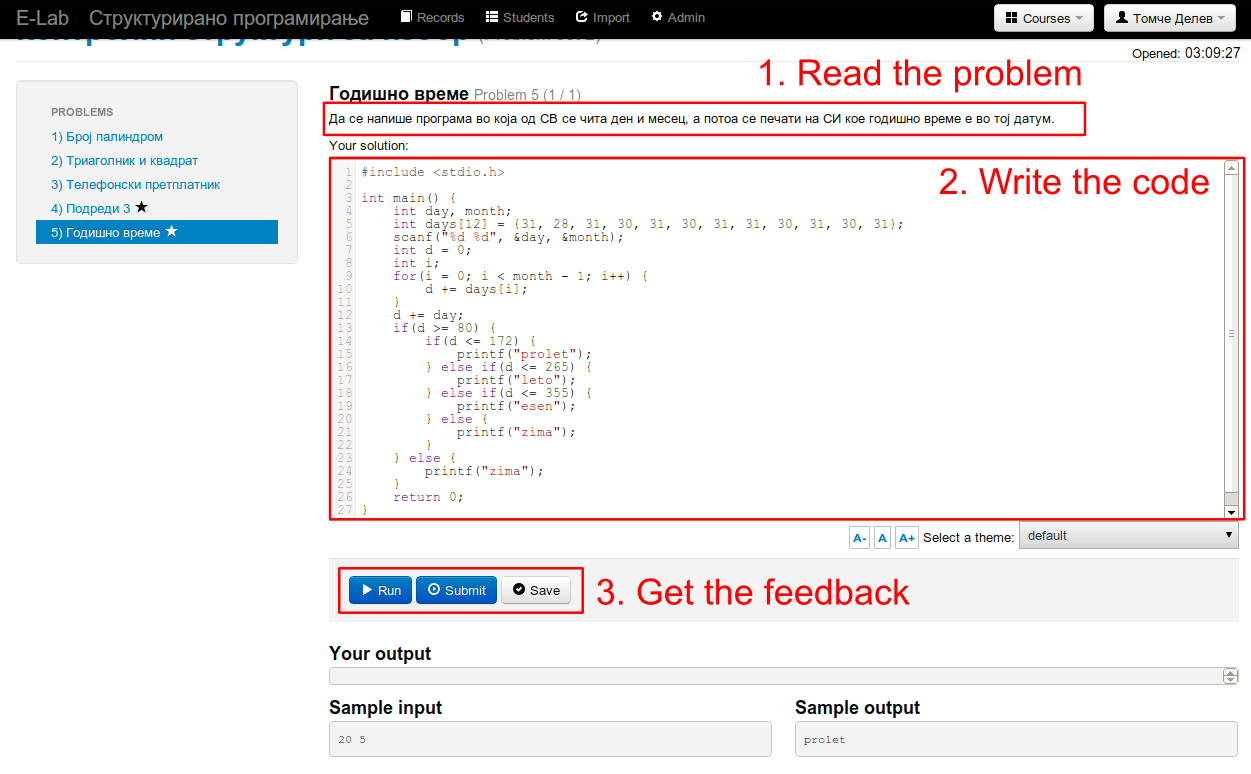
\includegraphics[width=.99\textwidth]{e-lab/user_screen}
\caption{The student screen trying to solve a problem.}
\label{fig:student_screen}
\end{figure}

According to this observation, the platform was designed in such a manner, so
that on a single screen students can work and accomplish all the phases involved
in solving the problems. As can be seen on figure \ref{fig:student_screen}, on
that single screen we have the problem text to be read, the web-based code editor to write the
solution and the actions pane, so they can run their solution and get instant
feedback in the output area. With this design we try to implement the extreme
apprenticeship method \cite{vihavainen2011extreme} which is based on a set of
values and practices that emphasize learning by doing, together with continuous feedback as the most
efficient means for learning programming.

\subsection{Authentication}

All users of the system are authenticated using the Central Authentication
System (CAS) which is used by all services at the faculty. With this mechanism
we can identify students and their solutions, and later use this identity to
export attendance and score records or check for plagiarism, malicious code or
other abusive usages.

\subsection{Problems design}

The central entities in the programming exercises are the programming problems.
Each problem is designed in two phases. In the first phase we define the problem
text, name and in some problems provide starter code. This information define
only the basis of the problem, so in the second phase we need to provide sample
input and output for the problem as an example, and at least one test case, also
in form of input and output data, so the solutions of the problem can be tested.
For each problem, we can also add contextual help or hints that can be helpful
for students to solve the problem.

\subsection{Automatic assessment}

Having limited resources in time and the identified difficulties that tutors and
instructors have trying to assess all of the student solutions to the given
problems makes the automatic assessment top priority in the platform. Since the
platform covers only introduction level courses in programming and algorithms,
most of the problems can be designed so they can be assessed by simple black-box
testing methodology. For each problem assignment the author provides a reference
solution, and using this solution the system automatically generates test cases.
Each test case consists of simple input and output text files. When the system
tests the solution, if it's compiled successfully, the executable is fed with
the input file and to be correct it should print out the same output as the
contents in the generated output file. One of the test cases is a sample and is
visible for the students, so they can better understand the problem. In our
implementation, each problem should have at least one test case and up to ten
test cases. This shouldn't be taken as a general rule, be our choice to limit
the number of test cases, was to be able to provide instant feedback. If we have
more test cases, then if their execution always results in time out (the program
doesn't end in a limited time), the user will need to wait this time out period
times the number of test cases.

\section{Architecture}

The overview of the system architecture can be seen on figure \ref{fig:architecture}, showing its
primary components. The data repository is the most interesting component of the
system. We propose a specific way of storing the problems and all the work from
the students by using a combination of database and file system. All the
relational data and meta-data of the problems such as the name, the problem set
it belongs, the text, are stored in relational database. The other part
containing the starter code, reference solution, help contents in mark-up text
and all the test cases in form of input and output text files are stored on the
file system. And finally, all of the students' solutions are stored solely on
the file system in organized directory structure. 

\begin{figure}
\centering
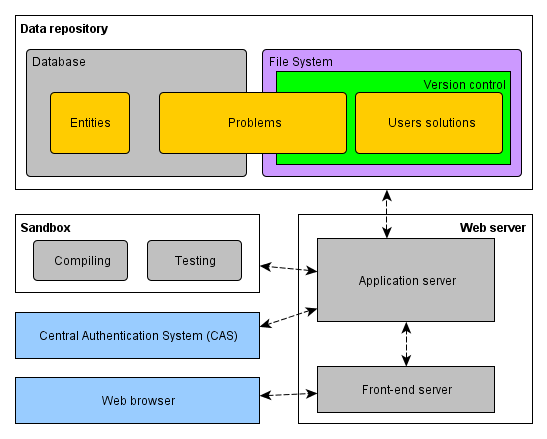
\includegraphics[width=.99\textwidth]{e-lab/architecture}
\caption{The E-Lab architecture.}
\label{fig:architecture}
\end{figure}

\subsection{Problems and solutions repository}

Almost all of the problems information and solutions are in form of simple text
or source code files. Very practical way of storing this kind of data is using
some kind of version control system. With this system we get features such as
management of the changes of the documents and full revision tracking
capabilities. The choice of Git, which is very fast distributed revision control
system, gives the system the reliability of the distributed repositories that
doesn't depend on single server.

\subsection{The client-server}

The system is a form of standard client-server web architecture. This
architecture allows the client, which is standard and web browser available on
all platforms, to run on virtually every PC in our computer lab environment.
This lowers the costs of maintenance of the computer labs, because no specific
software such as separate client software, compilers, IDEs or text editors
should be installed and maintained.

The web server is composed of two separate servers. The front-end web server is
a fast web server that serves as a fast proxy and load balancer to the
application server. The application server is Java server that uses a scalable
RESTfull architecture. The web application on this server follows the MVC
architectural pattern applied to the web architecture. The authentication of the
users is done on a central authentication server using HTTPS.

\subsection{Asynchronous jobs}

In our architecture as in most web based architectures, the web application
server is intended to work with very short requests. It uses a fixed thread pool
to process requests queued by the HTTP connector. To get optimum results, the
thread pool should be as small as possible. The typical optimum value for the
default pool size is the number of processors + 1.

That means that if a request is very long, such as waiting the execution of a
program that times out (for example 3 seconds), will block the thread pool and
penalize the application responsiveness. Of course, we could add more threads to
the pool, but it will result in wasted resources, and anyway the pool size will
never be infinite.

In the example when users submitting solutions that should be tested on 3 test
cases and each of these solutions times out (3 seconds), then the request will
last at least 9 seconds (3 test cases x 3 seconds each). When 10 users
simultaneously try to submit their solutions, the server will need at least 10
execution threads. This number is feasible, but if we want to have scalable
system that supports hundreds or more users submitting solutions, we need
different approach.

In these cases, our web framework allows us to temporarily suspend the request.
The HTTP request will stay connected, but the request execution will be popped
out of the thread pool and tried again later. We execute our long lasting
operations such as compiling, saving and executing in an asynchronous way. We
use for execution, something called asynchronous job, and while these jobs are
executing, the HTTP request is suspended and waits for the result to be
available. When the jobs are done with the execution the HTTP request resumes
and returns the result to the user.

\subsection{Sandboxed execution}

The system allows students to write, run and execute any kind of program code
that will be executed on a remote server. This can harm the server in many
undesirable ways. The malicious code can contain unprivileged read and write
access, can create fork bombs, allocate all the available memory or simply
consume all the processing power the server has. To control or prevent these
security issues all the execution is done in a “sandbox” environment. In this
sandbox each execution is limited by processing time and memory, and also
constrained in the number of processes it can fork.

\section{Detecting Plagiarism}

Source code plagiarism is a serious problem and we must make it very clear to
students that the automated system will not be tolerating any kind of source
code plagiarism. The large number of submissions makes it very difficult to
manually check for evidences of plagiarism in all possible combinations of
solutions. We must use some automatic system for plagiarism detection. Automatic
plagiarism detection has been the subject of many studies
\cite{baker1995finding}, \cite{clough2000plagiarism} and there are many systems
available online.

In the E-Lab system we incorporate one of these systems trying to prevent and
detect plagiarism cases. We use the MOSS system developed by Alex Aiken at UC
Berkeley \cite{aiken2005moss}. The “Measure Of Software Similarity” system makes
it possible to objectively and automatically check all problem solutions for evidence of
plagiarism or simple copying. MOSS works with programming languages like C, C++,
Java, Python and many others. The strategy in our system is to present it very
clear to the students, that their solutions will be checked for plagiarism
against all solutions submitted by other students. Some of the introduction
level problems have very short and simple solutions. We exclude these
submissions from plagiarism detection, because the nature of these problems
makes it very difficult to write conceptually different solutions.

\section{Conclusion}

With the development and introduction of the E-Lab system we try to address many
organizational aspects of the lab exercises from introduction level programming
courses at our faculty. We try to simplify and improve the process of creating
and managing simple programming problems. The system is focused on the student
and his work and the role of the instructors is to motivate and help students to
write working solutions for most of the problems.

The implementation of the central and reliable data repository should also bring
many advantages. It contains all student's solutions and other important
information such as the time when problems were solved or time needed to solve.
All the solutions are version controlled, so we can track and analyze the stages
in solving and fixing bugs from beginner programmer perspective. All these
records, provides us with valuable information from the learning process of the
students. From this data, very easy we can extract information such as student's
attendance records and final scores.

With this system, we are not trying to solve all the organizational and
educational problems or entirely exclude the human factor. E-Lab is developed to
help with these problems and create modern environment that will motivate and
support students work in programming.

\bibliographystyle{splncs03}

\bibliography{e-lab}

\end{document}
